\documentclass{scrreprt}

\usepackage[utf8]{inputenc}
\usepackage[ngerman]{babel}
\usepackage{amsmath}
\usepackage{amsthm}
\usepackage{amssymb}
\usepackage{mathtools}

\parskip 12pt

\begin{document}

\tableofcontents

\chapter{Einleitung}
\section{Problembeschreibung}
Bei synchronen Flow-Shop-Problemen handelt es sich um Produktions\-planungs\-probleme,
bei denen die zu produzierenden Güter (Jobs) z.B. auf einer zyklisch angeordneten Produktionsanlage
produziert werden. Die Produktionsanlage be\-steht aus $m$ Stationen, die sich mit der Anlage drehen.
Außen, um die Anlage herum, befinden sich $m$ fortlaufend nummerierte fixierte Maschinen $M_1,\ldots,M_m$, die die einzelnen Produktionsschritte durchführen.
Dabei handelt es sich bei Maschine $M_1$ um das Einlegen des Jobs in die Anlage und bei Maschine $M_m$ um die Entnahme des fertigen Produkts.
Durch Rotation der Anlage werden die Stationen mit den auf ihnen befindlichen Jobs zur jeweils nächsten Maschine transportiert.
Die Reihenfolge, in der alle Jobs die Maschinen durchlaufen müssen ist also fest vorgegeben.
In Abbildung \ref{abb:Anlage} ist eine solche zyklische Anlage dargestellt.
\begin{figure}
    \begin{center}
        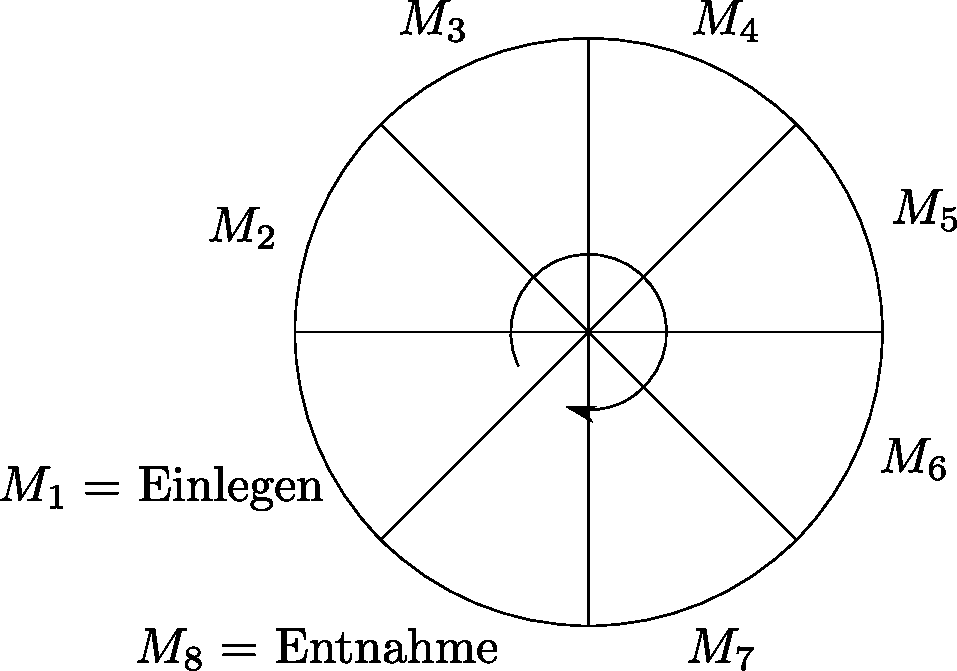
\includegraphics[width=.6\textwidth]{graphics/anlage.pdf}
    \end{center}
    \caption{
        \label{abb:Anlage}
        Kreisförmige Anlage mit $m=8$ Maschinen.
    }
\end{figure}
Eine Rotation darf immer nur dann stattfinden, wenn alle Maschinen ihren Produktionsschritt an ihrem aktuellen Job
durchgeführt haben. Auf diese Weise können die Jobs, im Gegensatz zum klassischen (asynchronen) Flow-Shop, 
immer nur \textit{synchron} zur nachfolgenden Maschine gelangen.
Die Zeit, die zwischen zwei Rotationen vergeht, wird als \textit{Zykluszeit} bezeichnet.

Die zu produzierenden Jobs sind gegeben durch die Menge $J=\{j_1,\ldots,j_n\}$ 
und die Prozesszeiten von Job $j$ auf Maschine $M_i$ sind durch $p_{ij}$ gegeben.
Eine Beispielinstanz mit $n=5$ und $m=3$ ist in Tabelle \ref{abb:Bsp} zu sehen.
\begin{figure}
    \begin{center}
        \begin{tabular}{c|ccc}
            & $M_1$ & $M_2$ & $M_3$ \\ \hline
            $j_1$ & 4 & 6 & 5 \\
            $j_2$ & 1 & 5 & 6 \\
            $j_3$ & 2 & 5 & 4 \\
            $j_4$ & 5 & 2 & 4 \\
            $j_5$ & 4 & 5 & 4
        \end{tabular}
    \end{center}
    \caption{
        \label{abb:Bsp}
        Beispielinstanz mit 5 Jobs und 3 Maschinen. Die Werte in der Tabelle sind die Prozesszeiten $p_{ij}$.
    }
\end{figure}
\begin{figure}
    \begin{center}
        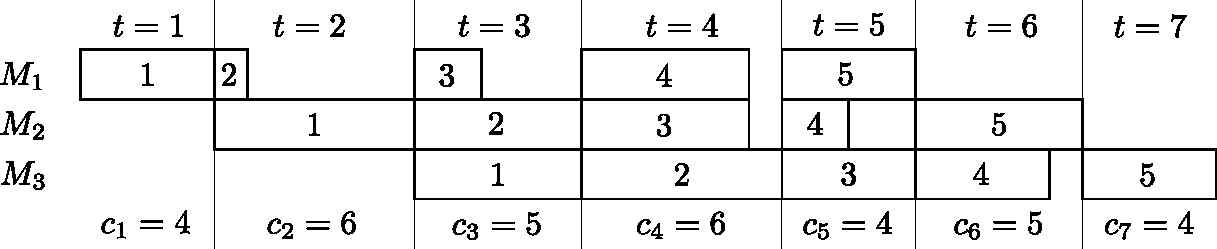
\includegraphics[width=.8\textwidth]{graphics/bspinit.pdf}
    \end{center}
    \begin{center}
        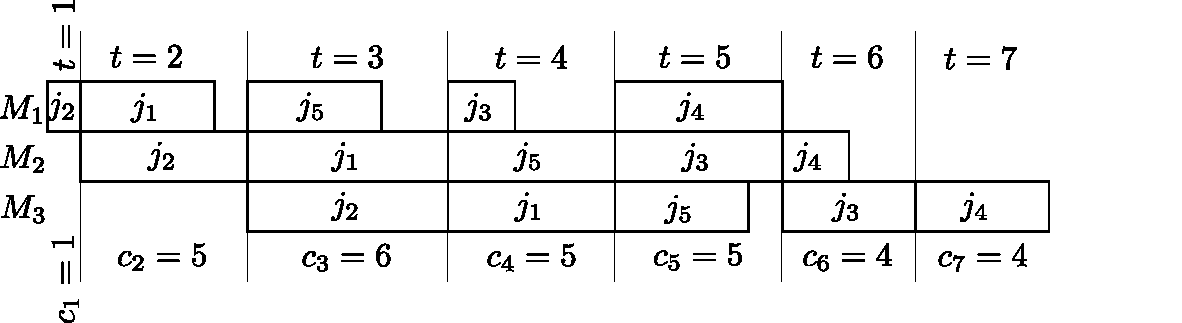
\includegraphics[width=.8\textwidth]{graphics/bspopt.pdf}
    \end{center}
    \caption{
        \label{abb:gantt}
        Gantt-Diagramme der initialen Reihenfolge von Beispiel \ref{abb:Bsp} mit $C_{\max}=34$
        und einer optimalen Reihenfolge mit $C_{\max}=30$.
    }
\end{figure}
Ziel ist es, eine Permutation $\pi$ der Jobs zu erstellen, die die gesamte Produktionsdauer minimiert.
Diese Zielfunktion wird mit $C_{\max}$ bezeichnet.
Die Beispielinstanz \ref{abb:Bsp} ist in Abbildung \ref{abb:gantt} als Gantt-Diagramm aufgetragen.
Oben sind die Jobs in der initialen Reihenfolge und unten in einer bezüglich $C_{\max}$ optimalen Reihenfolge.
Die Zykluszeiten $c_t$ mit $1\leq t\leq n+m-1$ berechnen sich wie folgt:
\[ c_t = \max_{i=\max\{1,t-n+1\}}^{\min\{t,m\}} p_{i\pi_{t-i+1}} \]
Die Zielfunktion lässt sich also durch $C_{\max} = \sum_{t=1}^{n+m-1} c_t$ berechnen.
Andere Zielfunktionen werden in dieser Masterarbeit nicht betrachtet.

Eine Teilmenge $D \subseteq \{M_1,\ldots,M_m\}$ der Maschinen heißt \textit{dominierend}, wenn 
\[ p_{dj} \geq p_{ej} \quad \forall j\in J, d\in D, e\not\in D \] 
ist. Die Prozesszeiten aller Jobs auf dominierenden Maschinen sind also immer mindestens so groß wie die Prozesszeiten auf den restlichen Maschinen.
Treten dominierende Maschinen auf, müssen für die Berechnung der Zykluszeiten die Prozesszeiten auf den übrigen Maschinen also nicht betrachtet werden.

Zusätzlich benötigen die Jobs Ressourcen aus einer Menge $R$, um in die Stationen eingelegt werden zu können. Diese Ressourcen können erst nach
Fertigstellung eines Jobs, also nachdem er an Maschine $M_m$ aus der Anlage genommen wurde, wiederverwendet werden.
Sie sind allerdings nur in begrenzter Zahl vorhanden und im Allgemeinen ist nicht jede Ressource für jeden Job geeignet.
Für $j\in J$ sei $\rho_j\subseteq R$ die Menge der Ressourcen, die für $j$ geeignet ist.
Umgekehrt sei für $r\in R$ mit $\iota_r\subseteq J$ die Menge der Jobs bezeichnet, für die $r$ geeignet ist.
An Maschine $M_1$ kann es daher notwendig sein, vor dem Einlegen des nächsten Jobs die Ressource zu wechseln, 
wenn auf der entsprechenden Station zuvor Job $j\in J$ mit Ressource $r\in\rho_j$ fertiggestellt wurde 
und nun Job $j'\not\in\iota_r$ eingelegt werden soll.

Für die Ressourcen können folgende Situationen auftreten:
\begin{itemize}
    \item Alle Ressourcen sind für alle Jobs geeignet, also $\rho_j=R$ für alle $j\in J$.
    \item Die Jobs lassen sich in disjunkte Gruppen unterteilen, so dass für alle Jobs aus einer Gruppe dieselbe Ressourcenmenge geeignet ist.
        Wenn also $\rho_i \cap \rho_j \neq \emptyset$, dann folgt $\rho_i=\rho_j$.
    \item Die Ressourcenmengen bilden Hierarchien. 
        D.h., wenn $\iota_q \cap \iota_r \neq \emptyset$, dann folgt $\iota_q \subseteq \iota_r$ oder $\iota_r \subseteq \iota_q$.
    \item Die $\rho_j$ sind beliebige Teilmengen von $R$.
\end{itemize}%
Neben dem Wechsel von Ressourcen, der zusätzliche Zeit in Anspruch nimmt, können auch andere Formen von \textit{Rüstkosten}
auftreten. Z.B. kann es sein, dass an einer Station zunächst einige Umstellungen vorgenommen werden müssen, bevor der
neue Job eingelegt werden kann. Die Jobs können in Familien $\mathcal{F}$ eingeteilt werden, so dass beim Übergang
zwischen zwei Jobs aus den Familien $f$ und $g$ die Rüstkosten $s_{fg}$ auftreten.
Diese Rüstkosten können 
\begin{itemize}
    \item sowohl vom Vorgänger als auch vom Nachfolger abhängig sein ($s_{fg}$), 
    \item nur vom Nachfolger abhängig sein ($s_{fg} = s_{g}$) oder
    \item konstant sein ($s_{fg} = s > 0$).
\end{itemize}%
Dabei wird $s_{ff} = 0$ angenommen für alle $f\in\mathcal{F}$, dass also keine Rüstkosten innerhalb einer Familie auftreten.
Wenn Rüstkosten auftreten, soll nicht mehr nur die Summe aller Zykluszeiten minimiert werden, sondern zusätzlich noch die Summe aller auftretenden Rüstkosten.
Diese Zielfunktion lässt sich als 
\[ \min\left(C_{\max}+\sum_{f,g\in\mathcal{F}}s_{fg}y_{fg}\right) \] 
formulieren, wobei die Variablen $y_{fg}$ angeben, wie oft die Rüstkosten $s_{fg}$ von einem Job aus Familie $f$ zu einem aus Familie $g$ auftreten.

\begin{figure}
    \begin{center}
        \begin{tabular}{c|ccccc}
            & $j_1$ & $j_2$ & $j_3$ & $j_4$ & $j_5$ \\ \hline
            $j_1$ & 0 & 8 & 5 & 9 & 4\\
            $j_2$ & 6 & 0 & 6 & 8 & 8\\
            $j_3$ & 4 & 7 & 0 & 5 & 4\\
            $j_4$ & 5 & 7 & 8 & 0 & 9\\
            $j_5$ & 4 & 5 & 8 & 9 & 0
        \end{tabular}
    \end{center}
    \caption{
        \label{abb:BspRes}
        Rüstkosten für die Beispielinstanz aus Tabelle \ref{abb:Bsp}.
        Beispielsweise treten Rüstkosten von $6$ auf, wenn von $j_2$ auf $j_1$ gewechselt werden muss.
    }
\end{figure}
In Abbildung \ref{abb:BspRes} ist eine mögliche Rüstkostentabelle für das Beispiel aus \ref{abb:Bsp} gegeben.
Die initiale Reihenfolge und eine optimale sind in Abbildung \ref{ganttres} als Gantt-Diagramm dargestellt.
\begin{figure}
    \begin{center}
        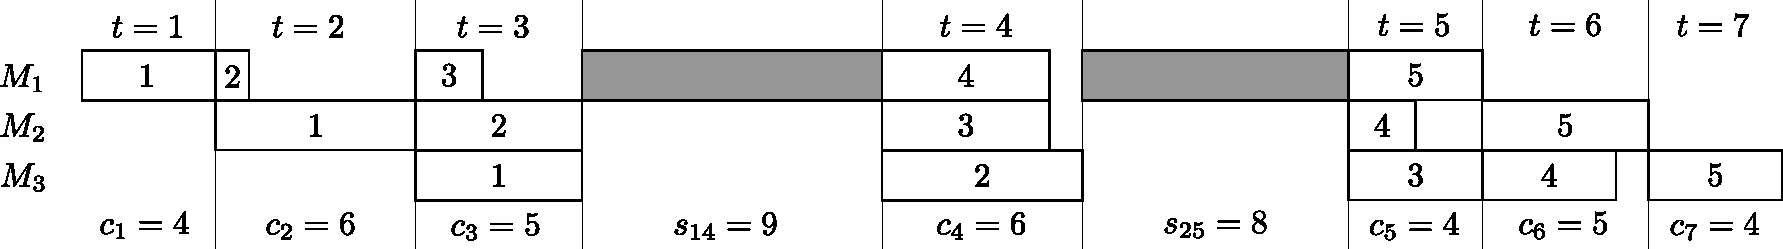
\includegraphics[width=\textwidth]{graphics/bspresinit.pdf}
    \end{center}
    \begin{center}
        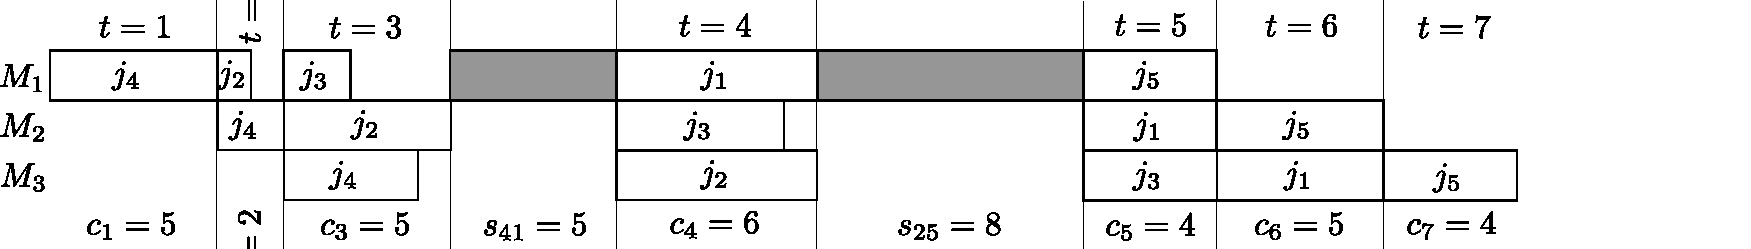
\includegraphics[width=\textwidth]{graphics/bspresopt.pdf}
    \end{center}
    \caption{
        \label{abb:ganttres}
        Initiale und eine optimale Lösung als Gantt-Diagramme für das Beispiel aus \ref{abb:Bsp} erweitert um Rüstkosten aus \ref{abb:BspRes}.
    }
\end{figure}

Insgesamt gilt es, neben der Reihenfolge $\pi$ auch ein Mapping $f:J\rightarrow R$ zu finden, 
das jedem Job $j\in J$ eine Ressource $r\in\rho_j$ zuweist und folgenden Ansprüchen genügt:
\begin{itemize}
    \item $f$ muss zulässig sein in dem Sinne, dass beim Einlegen jedes Jobs $j\in J$ eine Ressource $r\in\rho_j$ verfügbar ist
        (d.h., dass $r$ sich nicht gerade an anderer Stelle in der Anlage befindet).
    \item $f$ und $\pi$ zusammen sollen optimal sein in dem Sinne, dass die Summe aus den durch $\pi$ und $f$ definierten Zykluszeiten und 
        Rüstkosten minimal ist.
\end{itemize}

\section{Motivation}
In \cite{...} wurde gezeigt, dass schon das Optimieren bezüglich $C_{\max}$, also ohne Ressourcen und Rüstkosten, $\mathcal{NP}$-schwer ist.
Versuche, dieses Problem -- oder auch einige Spezialfälle davon -- mit ganzzahliger linearer Programmierung optimal zu lösen, waren nur für sehr kleine Instanzen mit
$n<30$ in hinnehmbarer Zeit erfolgreich, was weit hinter praktischen Anforderungen zurückliegt (vgl. Abschnitt \ref{subsec:LineareProgrammierung}. 
Aufgrund der Komplexität des Gesamtproblems sollen in dieser Arbeit zwei Dekompositionsansätze verfolgt werden:
\begin{enumerate}
    \item Zunächst wird eine Reihenfolge $\pi$ aufgestellt, ohne Ressourcen und Rüstkosten zu betrachten, so dass $C_{\max}$ möglichst gut ist.
        Anschließend wird ein Mapping $f$ basierend auf $\pi$ erstellt, möglichst ohne nachträgliche Änderung an $\pi$ vorzunehmen.
    \item Es wird zuerst ein Mapping $f$ erstellt, so dass die Ressourcen zulässig zugewiesen sind und die durch die Ressourcenwechsel verursachten Rüstkosten minimal sind.
        Anschließend werden, ohne $f$ zu verändern, die Jobs so in einer Reihenfolge $\pi$ angeordnet, dass die Zykluszeiten möglichst minimal sind.
\end{enumerate}%
Beide Ansätze liefern natürlich im Allgemeinen keine optimalen Lösungen, da jeweils getrennt bezüglich $\pi$ und $f$ optimiert wird,
obwohl die optimale Lösung von beiden zusammen abhängig ist.
Außerdem sind selbst die aus den Ansätzen resultierenden Teilprobleme teilweise noch $\mathcal{NP}$-schwer.
Beispielsweise ist bei Ansatz (1) das Berechnen einer $C_{\max}$-optimalen Reihenfolge $\pi$ in dem Spezialfall,
dass es nur eine dominierende Maschine gibt trivial, da $C_{\max}$ bei jeder Reihenfolge identisch ist,
und wenn es genau zwei benachbarte dominierende Maschinen gibt,
ist es mit dem Algorithmus von Gilmore und Gomory \cite{...} in Polynomialzeit lösbar.
Bei der anschließenden Zuweisung von Ressourcen ist noch unbekannt, ob ein polynomieller Algorithmus existiert.
%Dies herauszufinden ist eines der Ziele dieser Arbeit.

Je nachdem, ob die Rüstkosten die Zykluszeiten dominieren oder umgekehrt, ist Ansatz (2) bzw. Ansatz (1) vielversprechender.

\section{Bisherige Ansätze}
\label{sec:bisherigeAnsaetze}
Als weitere Motivation für die Dekompositionsansätze dient folgendes Mixed Integer Linear Program (MIP):
\begin{align}
    \text{min} \quad \sum_{t=1}^{n+m-1} &c_t + \sum_{j=1}^n \sum_{h=1}^n s_{jh} y_{jh} \label{allmip:obj}\\
    \text{s.t.}\quad \sum_{k=1}^n x_{jk} &= 1 & j\in N \label{allmip:1}\\
                     \sum_{j=1}^n x_{jk} &= 1 & k\in N \label{allmip:2}\\
    c_t &\geq \sum_{j=1}^n p_{t-k+1,j} \cdot x_{jk} & t\in T, k=\max\{1,t-m+1\},\ldots,\min\{n,t\} \label{allmip:3}\\
    y_{jh} + 1 &\geq x_{j,k-m} + x_{hk} & j,h\in N, k=m+1,\ldots,n \label{allmip:4}\\
    c_t &\geq 0 & t\in T \\
    x_{jk} &\in \{0,1\} & j,k\in N \\
    y_{jh} &\in \{0,1\} & j,h\in N
\end{align}
$N$ ist die Indexmenge der Jobs, also $N=\{1,\ldots,n\}$ und $T=\{1,\ldots,n+m-1\}$ ist die Indexmenge der Zykluszeiten.
Die Binärvariablen $x_{jk}$ geben an, an welcher Position $k$
sich Job $j$ befindet. Es gilt $x_{jk}=1$ genau dann, wenn $j$ an
Position $k$ ist. Die Nebenbedingungen \ref{allmip:1} und \ref{allmip:2}
stellen sicher, dass sich jeder Job an genau einer Position befindet und 
dass sich an jeder Position genau ein Job befindet.
In Nebenbedingung \ref{allmip:3} werden die Zykluszeiten bestimmt.
Den Binärvariablen $y_{jh}$ wird in Nebenbedingung \ref{allmip:4} folgende
Bedeutung gegeben: $y_{jh}=1$, wenn Job $j$ genau $m$ Positionen
vor Job $h$ in $\pi$ liegt.
In der Zielfunktion \ref{allmip:obj} wird dann die Summe aus allen
Zykluszeiten gebildet und die Summe aller Rüstkosten $s_{jh}$, die beim
Übergang von Job $j$ zu $h$ auftreten.

Obwohl in diesem MIP nicht die Verfügbarkeiten von Ressourcen beachtet werden,
benötigt es schon bei $n=20$ mehrere Stunden zum Finden der optimalen Lösung.
Es ist also für Instanzen mit mehreren Tausend Jobs nicht geeignet.
Aufgrund dieser Tatsache ist eine heuristische Herangehensweise an 
synchrone Flow-Shop-Probleme mit Ressourcen und Rüstkosten eine gute Alternative.


\chapter{Der erste Dekompositionsansatz}
Beim ersten Dekompositionsansatz wird zunächst eine (möglichst gute) Jobreihenfolge $\pi$ bestimmt.
Dabei werden Ressourcen und Rüstkosten außer Acht gelassen. 
Es wird also zunächst ausschließlich $C_{\max}$ optimiert. Anschließend wird ein Mapping $f$ aufgestellt,
so dass Ressourcen nur dann eingeplant werden, wenn sie auch zur Verfügung stehen, und darüber hinaus
möglichst selten ausgetauscht werden müssen, so dass geringe Rüstkosten auftreten.

In Abschnitt \ref{sec:BerechnenEinerJobreihenfolge} werden einige exakte und heuristische Verfahren für die
Berechnung einer $C_{\max}$-optimalen Reihenfolge $\pi$ vorgestellt, was im Allgemeinen $\mathcal{NP}$-schwer ist.
Anschließend werden in Abschnitt \ref{sec:ZuweisungVonRessourcen} Verfahren vorgestellt, die ein möglichst gutes Mapping $f$ erzeugen.
Dabei wird speziell darauf eingegangen, ob mit der gegebenen Reihenfolge $\pi$ und den gegebenen Ressourcen
überhaupt eine zulässige Lösung möglich ist, und, wie dann ggf. die Zulässigkeit durch nachträgliche Änderungen an $\pi$
erzeugt werden kann.

\section{Berechnen einer Jobreihenfolge}
\label{sec:BerechnenEinerJobreihenfolge}
\subsection{Gilmore Gomory}
Der Algorithmus von Gilmore und Gomory \cite{...} löst in $\mathcal{O}(n\log n)$ einen speziellen Fall des gerichteten Travelling-Salesman-Problems (TSP),
bei dem alle Knoten zwei Parameter $x,y$ haben und die Kantenkosten $c_{ij}$ zwischen je zwei Knoten $i$ und $j$ nur vom $x$-Wert von $i$
und vom $y$-Wert von $j$ abhängig sind.

Diese Situation liegt beim synchronen Flow-Shop vor, wenn es nur zwei benachbarte dominierende Maschinen gibt.
O.B.d.A seien dies $M_1$ und $M_2$.
Jobs können durch Knoten repräsentiert werden und die beiden Prozesszeiten auf den dominierenden Maschinen liefern die Parameter $x$ und $y$. 
Der Abstand zwischen zwei Knoten entspricht dann der Zykluszeit, die die entsprechenden Jobs verursachen, wenn sie nebeneinander liegen.
Die Berechnung der Zykluszeiten vereinfacht sich hier zu
$c_t = \max \{p_{2\pi_{t-1}},p_{1\pi_t}\}$ für $2\leq t\leq n$.
Sie sind also für je zwei Jobs $\pi_{t-1},\pi_{t}$ nur noch von der Prozesszeit des vorderen Jobs auf der zweiten Maschine ($p_{2\pi_{t-1}}$) 
und der Prozesszeit des hinteren Jobs auf der ersten Maschine ($p_{1\pi_t}$) abhängig.

Auf die Funktionsweise des Algorithmus soll in dieser Arbeit nicht näher eingegangen werden.
Eine Anwendung des Algorithmus von Gilmore und Gomory als Heuristik für ein Problem mit mehreren dominierenden Maschinen wird in
\ref{subsubsec:ggHeuristik} beschrieben.


\subsection{Ganzzahlige Lineare Programmierung}
\label{subsec:LineareProgrammierung}
Zum Finden einer $C_{\max}$-optimalen Lösung dieses Teilproblems wurde folgendes MIP aufgestellt.
Es ist identisch mit dem MIP in Abschnitt \ref{sec:bisherigeAnsaetze} bis auf die Nichtberücksichtigung der Rüstkosten.
\begin{align}
    \text{min} \quad \sum_{t=1}^{n+m-1} &c_t \\
    \text{s.t.}\quad \sum_{k=1}^n x_{jk} &= 1 & j\in N \\
                     \sum_{j=1}^n x_{jk} &= 1 & k\in N \\
    c_t &\geq \sum_{j=1}^n p_{t-k+1,j} \cdot x_{jk} & t\in T, k=\max\{1,t-m+1\},\ldots,\min\{n,t\} \\
    c_t &\geq 0 & t\in T \\
    x_{jk} &\in \{0,1\} & j,k\in N
\end{align}
Dieses MIP liefert für Instanzen mit $n\leq 30$ eine optimale Lösung in unter einer Stunde.
Diese Laufzeiten sind zwar schon deutlich besser als die Variante mit Rüstkosten in Abschnitt \ref{sec:bisherigeAnsaetze},
bei größeren Instanzen ist dieser Zeitaufwand allerdings immer noch nicht praktikabel. 

Für Instanzen mit $n\leq 500$ ist die beste nach einer halben Stunde gefundene Lösung in ihrer Güte vergleichbar mit den Heuristiken,
die in Unterabschnitt \ref{subsec:HeuristischeVerfahren} vorgestellt werden (für einen Vergleich s. \ref{subsec:VergleichDerHeuristiken}).
In diesem Sinne kann dieses MIP daher ebenfalls als Heuristik betrachtet werden.


\subsection{Heuristische Verfahren}
\label{subsec:HeuristischeVerfahren}
Aufgrund der $\mathcal{NP}$-Schwere der Optimierung von $C_{\max}$ im allgemeinen Fall und der schlechten Laufzeit des MIPs aus Abschnitt \ref{subsec:LineareProgrammierung}
bei Instanzen realer Größe werden hier einige heuristische Ansätze zur Berechnung von $\pi$ vorgestellt.

\subsubsection{Non-Full-Schedule-Heuristik}
Diese Heuristik ist eine konstruktive Greedy-Heuristik, die Schritt für Schritt einen Job an $\pi$ anhängt, beginnend mit einer leeren Reihenfolge.
Sie arbeitet ähnlich wie die Nearest-Neighbor-Heuristik beim TSP.
In jeder Iteration werden alle noch verbleibenden Jobs bewertet und der Job mit der besten Bewertung wird an $\pi$ angehängt.
Die Heuristik benötigt also genau $n$ Iterationen.
Die Bewertungsfunktion betrachtet die letzten $m-1$ Zykluszeiten der noch nicht fertigen Reihenfolge, 
wobei die Zykluszeiten am Anfang bei einer noch leeren Reihenfolge als $0$ angenommen werden.
Für jeden Job $j$, der noch nicht in $\pi$ ist, werden diese $m-1$ Zykluszeiten mit den ersten $m-1$ Prozesszeiten von $j$ verglichen.
Die Idee ist, dass diese möglichst übereinstimmen sollten. Ist eine Prozesszeit sehr viel größer als die aktuelle Zykluszeit,
zu der sie hinzugefügt werden würde, würde die Zykluszeit entsprechend um einen Wert $c_+$ ansteigen.
Ist umgekehrt die Zykluszeit sehr viel größer als die zugehörige Prozesszeit von $j$, dann würde diese kurze Prozesszeit verschenkt werden.
Die Differenz aus Zykluszeit und Prozesszeit wird mit $c_-$ bezeichnet.
Die Bewertungsfunktion berechnet für jeden Job die Summe aus den $m-1$ $c_+$-Werten.
Diese Summe ist die Bewertung für einen Job $j$. Der Job mit der kleinsten Bewertung wird an $\pi$ angehängt.
Falls mehrere Jobs eine optimale Bewertung haben, wird für diese Jobs als zweites Kriterium die Summe der $c_-$-Werte betrachtet.
Der Job, bei dem diese Summe am kleinsten ist, verschenkt am wenigsten Zeit und wird ausgewählt.
Das Vorgehen dieser Heuristik wird anhand der Beispielinstanz \ref{abb:Bsp} in Abbildung \ref{abb:nfsbsp} veranschaulicht.
\begin{figure}
    \begin{center}
%        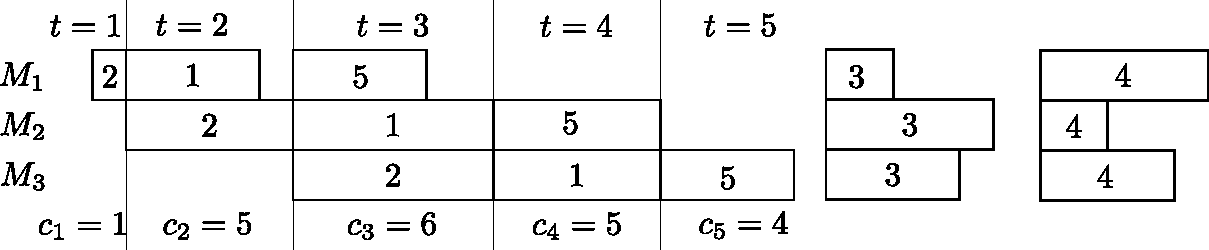
\includegraphics[width=.8\textwidth]{nfsbsp.pdf}
    \end{center}
    \caption{
        \label{abb:nfsbsp}
    }
\end{figure}

Da in jeder Iteration alle verbleibenden Jobs betrachtet werden und für jeden dieser Jobs $m-1$ Zeiten verglichen werden,
liegt die asymptotische Laufzeit dieser Heuristik in $\mathcal{O}(n^2m)$.

\subsubsection{Double Ended Non-Full-Schedule-Heuristik}
Diese Heuristik basiert auf der Non-Full-Schedule-Heuristik.
Der Unterschied besteht darin, dass $\pi$ nicht nur von vorne, sondern gleichzeitig auch von hinten zur Mitte hin aufgebaut wird.
Jeder noch nicht in $\pi$ enthaltende Job wird pro Iteration mit beiden Enden der bisherigen Reihenfolge verglichen.
Die Bewertungsfunktion für das hintere Ende arbeitet analog.
Es wird der beste Job für das vordere Ende und der beste für das hintere Ende gesucht und der mit der besseren Bewertung wird vorne bzw. hinten eingefügt.
Die asymptotische Laufzeit liegt hier ebenfalls in $\mathcal{O}(n^2m)$.

\subsubsection{Gilmore-Gomory-Heuristik}
\label{subsubsec:ggHeuristik}
Diese Heuristik wendet den Algorithmus von Gilmore und Gomory auf beliebige Instanzen an.
Es können zwei Fälle eintreten:
\begin{enumerate}
    \item Unter den dominierenden Maschinen $D$ gibt es zwei, die benachbart sind, also $\exists i\in\{1,\ldots,m\}, M,M'\in D$ mit $M=M_i$ und $M'=M_{i+1}$.
    \item Es gibt keine benachbarten dominierenden Maschinen.
\end{enumerate}
Wenn Fall (2) eintritt, werden alle $m$ Maschinen als dominierend angesehen, da dies für den Algorithmus keine Einschränkung darstellt.
Nun werden zwei benachbarte dominierende Maschinen gewählt.
O.B.d.A seien dies die Maschinen $M_1$ und $M_2$. Seien 
\begin{align} 
    d_{\min} &\coloneqq \min_{\substack{i\in \{1,2\} \\ j\in J}} p_{ij} \\
    e_{\max} &\coloneqq \max_{\substack{i\not\in \{1,2\} \\ j\in J}} p_{ij} \\
    K &\coloneqq \frac{e_{\max}}{d_{\min}} \text{,}
\end{align}
wobei $d_{\min}=0$ und daraus folgend $K=\infty$ erlaubt sind. 
Nun wird aus der gegebenen Instanz $I$ eine neue Instanz $I'$ erzeugt, die sich nur dadurch von $I$ unterscheidet, dass die Prozesszeiten
auf allen dominierenden Maschinen außer auf $M_1$ und $M_2$ mit $\frac{1}{K}$ skaliert werden, also
\begin{align}
    p'_{ij} \coloneqq \begin{cases} \frac{p_{ij}}{K} &\text{für } i\in D\setminus\{M_1,M_2\} \\ p_{ij} &\text{sonst.} \end{cases}
\end{align}
Auf diese Weise sind $M_1$ und $M_2$ in $I'$ die einzigen dominierenden Maschinen und folglich kann $I'$ mit dem Algorithmus von Gilmore und Gomory optimal gelöst werden.
Die resultierende Reihenfolge $\pi$ wird als heuristische Lösung für die ursprüngliche Instanz $I$ verwendet.

Da die Prozesszeiten der in $I'$ vernachlässigten dominierenden Maschinen sich um den Faktor $K$ von denen in $I$ unterscheiden, 
können sich die aus $\pi$ ergebenen Zykluszeiten von $I$ und $I'$ auch maximal um den Faktor $K$ unterscheiden:
\begin{align}
    c_t \leq K\cdot c'_t \quad \forall 1\leq t\leq n+m-1
\end{align}
Da die optimale Lösung von $I'$ eine untere Schranke für die optimale Lösung von $I$ ist, also $C'_{\max} \leq C_{\max}$, folgt für die Lösung $L_{GG}$ der
Gilmore-Gomory-Heuristik:
\begin{align}
    L_{GG} \leq K\cdot C'_{\max} \leq K\cdot C_{\max}
\end{align}
Die Gilmore-Gomory-Heuristik hat also eine relative Gütegarantie von $K$.
Zusätzlich kann bei der Wahl der zwei benachbarten dominierenden Maschinen der Parameter $K$ optimiert werden, indem Maschinen nicht zufällig gewählt werden,
sondern so, dass die $d_{\min}$- bzw. $e_{\max}$-Werte optimal sind (und somit auch $K$).

Das finden der geeigneten dominierenden Maschinen kann in $\mathcal{O}(nm)$ durchgeführt werden. 
Das Anpassen der Prozesszeiten der übrigen dominierenden Maschinen ist nur in der Theorie von Interesse.
Der Gilmore-Gomory-Algorithmus kann diese einfach ignorieren.
Die Gesamtlaufzeit beträgt daher $\mathcal{O}(nm + n\log n)$.

Für die weitere Analyse dieser Heuristik soll der Begriff der \textit{Semidominanz} eingeführt werden.
Die Semidominanz ist ein Maß dafür, wie weit eine Teilmenge von Maschinen davon entfernt ist, dominierend zu sein.
Eine Semidominanz von $0$ bedeutet, die Maschinen sind dominierend.
Für eine Teilmenge von Maschinen $D\subseteq\{M_1,\ldots,M_m\}$ sei 
\[d_{\min} = \min_{\substack{i:M_i\in D \\ j\in\{1,\ldots,n\}}} p_{ij}\] 
die kleinste ihrer Prozesszeiten, analog zur obigen Definition von $d_{\min}$.
Die Semidominanz ist dann definiert als
\[\mathcal{D}_{D} \coloneqq \sum_{i: M_i\not\in D} \sum_{j=1}^n \max\{0,p_{ij}-d_{\min}\} \text{.}\]
Unabhängig von der \textit{relativen} Gütegarantie $K$ liefert diese Heuristik auch eine \textit{absolute} Gütegarantie von $\mathcal{D}_{\{M_i,M_{i+1}\}}$, 
wenn $M_i$ und $M_{i+1}$ als benachbarte Maschinen ausgewählt werden.
Die Gilmore-Gomory-Heuristik liefert also besonders gute Näherungen, wenn zwei benachbarte Maschinen fast dominierend sind und nur wenige Prozesszeiten auf anderen
Maschinen dies verhindern.

\subsubsection{Nachbarschaftssuche}
Mit einer Nachbarschaftssuche können bereits existierende (nicht optimale) Reihenfolgen verbessert werden.
Mögliche Nachbarschaftsoperatoren sind
\begin{itemize}
    \item $\mathit{xch}_{ij}$: vertauscht die Jobs an den Positionen $i$ und $j$ miteinander,
    \item $\mathit{shift}_{ij}$: "`shiftet"' den Job an Position $i$ nach Position $j$. 
        Alle Jobs zwischen $i$ und $j$ rücken um eins nach links (falls $i<j$) bzw. nach rechts (falls $i>j$).
\end{itemize}
Auf Grundlage dieser Nachbarschfaften lassen sich außerdem z.B. Iterative Improvement, eine Tabu-Suche oder Simulated Annealing implementieren.

Im Rahmen dieser Arbeit wurde ein Simulated Annealing Algorithmus auf Grundlage der $\mathit{xch}_{ij}$-Nachbarschfaft implementiert.


\subsection{Vergleich der Heuristiken}
\label{subsec:VergleichDerHeuristiken}


\section{Zuweisung von Ressourcen}
\label{sec:ZuweisungVonRessourcen}
In diesem Abschnitt geht es darum, den Jobs in der Reihenfolge $\pi$, die in Abschnitt \ref{sec:BerechnenEinerJobreihenfolge} aufgestellt wurde,
Ressourcen zuzuweisen. An diese Zuweisung werden zwei Anforderungen gestellt:
\begin{enumerate}
    \item Die Zuweisung muss zulässig sein. Das heißt, ist eine Ressource einem Job zugewiesen, darf sie den nachfolgenden $m-1$ Jobs nicht mehr zugewiesen werden.
        Das Problem der Zulässigkeit einer Zuweisung wird im ersten Unterabschnitt \ref{subsec:ZulaessigkeitDerZuweisung} betrachtet.
    \item Die Zuweisung soll möglichst optimal sein. Wenn zwei Jobs, die im Abstand von $m$ in $\pi$ liegen, die selbe Ressource benutzen können,
        werden Rüstkosten eingespart, da die Ressource nicht ausgetauscht werden muss.
        Dieses Problem wird in Unterabschnitt \ref{subsec:OptimierungDerRessourcenzuweisung} diskutiert.
\end{enumerate}
Es ist natürlich möglich, dass bei gegebenem $\pi$ keine zulässige Zuweisung von Ressourcen möglich ist.
In diesem Fall muss $\pi$ nachträglich geändert werden, worauf in Unterabschnitt \ref{UnzulaessigeReihenfolgen} eingegangen wird.

\subsection{Zulässigkeit der Zuweisung}
\label{subsec:ZulaessigkeitDerZuweisung}
Abhängig davon, welche Ressourcen für welche Jobs geeignet sind, kann das Zulässigkeitsproblem unterschiedlich schwer zu lösen sein.
Folgende Situationen werden betrachtet:
\begin{itemize}
    \item Alle Ressourcen sind für alle Jobs geeignet (trivial, es müssen $m$ Ressourcen vorhanden sein).
    \item Die Ressourcenmengen sind disjunkt ($\rho_i\cap\rho_j \neq \emptyset \enspace \Rightarrow \enspace \rho_i = \rho_j$).
    \item Die Ressourcen sind für hierarchische Jobgruppen geeignet 
        ($\iota_q\cap\iota_r \neq \emptyset \enspace \Rightarrow \enspace \iota_q\subseteq\iota_r$ oder $\iota_r\subseteq\iota_q$).
    \item Die $\rho_i$ sind beliebige Teilmengen von $R$.
\end{itemize}

\subsubsection{Zulässigkeit bei disjunkten Ressourcenmengen}
Bei disjunkten Ressourcenmengen können die Jobs in Gruppen unterteilt werden, 
so dass zu jeder Jobgruppe eine für sie exklusive Menge an zulässigen Ressourcen zur Verfügung steht.
Für die Zulässigkeit reicht es aus, statt der Ressourcenmengen $\rho_i$ nur deren Größen $|\rho_i|$ zu betrachten
(bei der Optimierung der Zuteilung ist diese Vereinfachung nicht sinnvoll).
Mit einem Greedy-Algorithmus kann eine gegebene Reihenfolge $\pi$ dann auf Zulässigkeit überprüft werden:
Der Algorithmus durchläuft $\pi$ von vorne nach hinten.
Jede Jobgruppe erhält einen Counter, der mitzählt, wie viele Ressourcen momentan für sie zur Verfügung stehen.
Diese Counter werden zu Beginn mit $|\rho_i|$ initialisiert.
An jeder Position in $\pi$ wird der Counter der zugehörigen Jobgruppe dekrementiert.
Nach $m$ Schritten wird dieser Counter wieder inkrementiert.
Sollte ein Counter einmal negativ werden, gibt es keine zulässige Ressourcenzuteilung.

\subsubsection{Zulässigkeit bei hierarchischen Jobgruppen}
%Diese Situation kann mit einem ähnlichen Greedy-Algorithmus gelöst werden, wie bei disjunkten Ressourcenmengen.
%Die Ressourcen, die für eine Jobgruppe geeignet sind, können hier allerdings nicht als identisch angesehen werden,
%so dass es genügen würde, wieder nur die Anzahl der Ressourcen zu betrachten.
%Die Ressourcen unterscheiden sich dahingehend voneinander, dass sie für unterschiedlich viele andere Jobs ebenfalls geeignet sind.
%Der Greedy-Algorithmus muss so abgeändert werden, dass er jedem Job in $\pi$ immer die "`speziellste"' aktuell für diesen Job verfügbare Ressource zuweist.
%Soll einem Job $j$ eine Ressource zugeteilt werden, muss unter allen geeigneten Ressourcen $r\in\rho_j$, 
%wobei $r$ nicht schon einem anderen Job zugewiesen sein darf, diejenige mit minimalem $|\iota_r|$ ausgesucht werden.
%
%Dieser abgewandelte Greedy-Algorithmus ist korrekt, denn immer, wenn die Situation auftritt, dass für einen Job $j$ keine Ressource verfügbar ist,
%liegt das daran, dass alle potentiell geeigneten Ressourcen $\rho_j$ bereits an einen der $m-1$ direkten Vorgänger von $j$ vergeben worden sind.
%Sei $f$ das unvollständige Mapping, das der Algorithmus bis zu diesem Punkt aufgestellt hat.
%Sei $F\subseteq N$ die Menge der Vorgänger von $j$, denen eine Ressource $r\in\rho_j$ zugeteilt wurde.
%Angenommen, es existiert ein zulässiges Mapping $f'$, obwohl der Algorithmus $j$ keine Ressource zuweisen kann.
%Dann muss es einen Job $i\in F$ geben mit $f'(i)\not\in\rho_j$.
%Wegen der hierarchischen Eigenschaft muss entweder $\iota_{f'(i)}\subset\iota_{f(i)}$ sein oder $\iota_{f(i)}\subseteq\iota_{f'(i)}$.
%Da $f(i)\not\in\rho_j$ ist (und somit auch $j\not\in\iota_{f'(i)}$),
%muss hier $\iota_{f'(i)}\subset\iota_{f(i)}$ sein, denn sonst wäre $j\in\iota_{f(i)}\subseteq\iota_{f'(i)}$.
%Das wiederum bedeutet, dass auch der Algorithmus dem Job $i$ die speziellere Ressource $f'(i)$ zugewiesen hätte.
%Da er das aber nicht getan hat, muss er sie stattdessen einem der $m-1$ direkten Vorgänger von $i$ zugewiesen haben.
%Sei $h$ dieser Vorgänger von $i$.
%Es ist also $f(h)=f'(i)$ und somit $f'(h)\neq f'(i)$.


\subsubsection{Zulässigkeit bei beliebigen Ressourcenteilmengen}
Es ist nicht bekannt, ob das Problem, zu entscheiden, ob es bei gegebenem $\pi$ ein zulässiges Mapping $f$ gibt, 
$\mathcal{NP}$-vollständiges ist oder ob es einen polynomiellen Algorithmus gibt.

Es besteht allerdings die Vermutung, dass zumindest einen polynomiellen Algorithmus in $n$ gibt. Ein Indiz für diese Vermutung liefert folgendes MIP:
\begin{align}
    \text{max} \quad &0 \label{zulmip:obj} \\
    \text{s.t.}\quad \sum_{r\in\rho_i} x_{ir} &= 1 & i\in N \label{zulmip:1} \\
    x_{ir} + x_{jr} &\leq 1 & i\in N, j=i+1,\ldots,i+m-1 \, ,r\in\rho_i\cap\rho_j \label{zulmip:2} \\
    x_{ir} &\in \{0,1\} & i\in N, r\in\rho_i
\end{align}
Die Binärvariablen $x_{ir}$ geben hier an, ob dem Job $i$ die Ressource $r$ zugeteilt wird.
In diesem Fall ist $x_{ir}=1$ und sonst $x_{ir}=0$.
Die erste Nebenbedingung \ref{zulmip:1} bewirkt, dass jedem Job genau eine Ressource zugewiesen wird.
Durch die zweite Nebenbedingung \ref{zulmip:2} kann jede Ressource jeweils nur einmal an $m$ aufeinander folgende Jobs vergeben werden.
Eine Zielfunktion ist nicht notwendig, da die Zulässigkeit nur durch die Nebenbedingungen entschieden wird.
Mit diesem MIP können selbst sehr große Instanzen mit $n\approx 100000$ (allerdings mit $m\leq 8$) in weniger als einer Sekunde gelöst werden.

Nebenbedingung \ref{zulmip:2} verhindert immer nur für Paare von Jobs, deren Abstand kleiner als $m$ ist, dass ihnen die selbe Ressource zugewiesen wird.
Das ist für die Korrektheit des MIPs zwar ausreichend, durch zusätzliche Nebenbedingungen, die dasselbe für Tripel, Quadrupel, bis hin zu $m$-Tupeln verhindern,
können aber einige fraktionale Lösungen der Relaxation "`abgeschnitten"' werden.
Für ein $k$-Tupel von Jobs, die alle in einem Abschnitt von $\pi$ der Länge $m$ stehen, sieht diese zusätzliche Nebenbedingung so aus:
\begin{align}
    \sum_{l=1}^k x_{i_lr} \leq 1 \quad i_l\in N, i_1<i_2<\ldots<i_k<i_1+m, r\in\bigcap_{l=1}^k \rho_{i_l}
\end{align}
Für $k=2$ ist diese Nebenbedingung identisch mit \ref{zulmip:2}.
Wird sie für $k=3,\ldots,m$ zu obigem MIP hinzugefügt, so war bei allen bislang getesteten Instanzen die Relaxation bereits ganzzahlig.
Ein Beweis, dass dies tatsächlich bei allen Instanzen der Fall ist, ist noch nicht gelungen.
Gelingt er, ist bewiesen, dass es in polynomieller Zeit möglich ist, zu entscheiden, ob es für eine gegebene Jobreihenfolge $\pi$ und 
gegebene (beliebige) Ressourcenteilmengen $\rho_i$ möglich ist, allen Jobs eine Ressource zuzuweisen.


\subsection{Optimierung der Ressourcenzuweisung}
\label{subsec:OptimierungDerRessourcenzuweisung}
\textit{Soll dieser Abschnitt noch Bestandteil der Arbeit sein? Wenn ja, dann werde ich mich da zwischendurch immer mal wieder dransetzen,
bis eine Lösung gefunden ist. Ein echter Zeitplan ist hierfür schwierig.}

Bei hierarchischen oder beliebigen Jobgruppen eine optimale Zuweisung mit möglichst wenig Rüstkosten finden.
Dazu (falls möglich) einen polynomiellen Algorithmus angeben bzw. einen Beweis zur $\mathcal{NP}$-Vollständigkeit.

\section{Unzulässige Reihenfolgen}
\label{UnzulaessigeReihenfolgen}
Für den Fall, dass für eine gegebene Reihenfolge $\pi$ kein zulässiges Mapping $f$ erstellt werden kann, muss $\pi$ nachträglich verändert werden.

\subsection{Nachbarschaftssuche}

\textit{Anfang August hiermit anfangen.}

Nachbarschaftenssuchen formulieren, die eine unzulässige Reihenfolge reparieren, so dass sie dann zulässig ist.
Dabei soll die Reihenfolge möglichst wenig von ihrer Optimalität einbüßen.

\subsection{Andere Ansätze}
Platzhalter, falls noch andere Ideen aufkommen.






\chapter{2. Dekompositionsansatz}
\section{Ressourcenzuweisung}
\textit{Dieser Abschnitt muss auch nur noch ausformuliert werden.}

Generell auf bekannte Laufzeitschranken und Verfahren für die Ressourcenzuweisung kurz eingehen.
Davon speziell erklären, wie mit Binpacking eine minimale Anzahl an Rüstkosten erreicht werden kann für $s_{fg}=s$.


\section{Zulässigkeit der Zuweisung}
\textit{Bis Mitte Juli sollte die Lösung hier erarbeitet sein.}

Folgende Fragen diskutieren und idealer Weise beweisen:
Gibt es unzulässige Lösungen beim Binpacking? Wenn ja, wie lassen sie sich reparieren?


\section{Anordnung der Jobgruppen}
\subsection{MIP mit fixierten Bins}
Vorstellung des MIPs mit fixierten Bins mit $s_{fg}=s$. Vorstellung einiger Laufzeiten. 
\textit{MIP steht. Evtl müssen noch einige Laufzeiten gemessen werden.}

Außerdem die erweiterte Formulierung auf allgemeine $s_{fg}$ und Diskussion.
\textit{MIP sollte bis Ende Juli formuliert und Laufzeiten gemessen sein.}

\subsection{MIP mit freien Bins}
\label{subsec:mipfreibins}
\textit{Muss nur noch aufgeschrieben werden. Evtl. noch ein paar Laufzeiten messen.}

Vorstellung des MIPs mit freien Bins. 
Die Laufzeit ist sehr viel schlechter, die primale Lösung ist aber meist schon nach kurzer Zeit besser als beim MIP mit fixierten Bins.

\subsection{Mehrere fixierte Reihenfolgen}
\textit{Jetzt damit anfangen. Wahrscheinlich bis Mitte August.}

Basierend auf den Erkenntnissen aus \ref{subsec:mipfreibins} das MIP mit fixierten Bins für mehrere Binreihenfolgen laufen lassen.
Um nicht sämtliche Binreihenfolgen durchprobieren zu müssen,
ggf. mit bipartitem gewichteten Matching ein lokales Optimum zwischen zwei Bins suchen und daraus eine "`gute"' Binreihenfolge erstellen.


\chapter{Messergebnisse und Vergleiche}
\textit{Anfang September anfangen, soweit Messergebnisse vorliegen.}

Obwohl in den vorherigen Kapiteln schon einige Laufzeiten vorgestellt werden, hier nochmal eine Zusammenfassung und insbesondere ein Vergleich
zwischen den beiden Dekompositionsansätzen. Sowohl echte Instanzen als auch generierte. 
Dabei ggf. auf Methoden zur Instanzengenerierung eingehen und diese bewerten?

\end{document}
